\documentclass[12pt,a4paper]{article}
\usepackage{polski}
\usepackage{wmstitle_lic}
\usepackage{graphicx}
\usepackage{color}
\usepackage{mathtools}

\newtheorem{df}{Definicja}[section]
\newtheorem{pr}{Przyk{\l}ad}[section]

\begin{document}

\title{Hipoteza \v Cernego}
\author{Sylwia Klimkiewicz, Adam Jamka}
\promotor{Wit Fory\'s}
\nralbumu{276782, 276765}
\maketitle


%% SEKCJA 1 Podstawowe definicje
\section{Podstawowe definicje.}
%% def 1.1
\begin{df} 
Grafem nazywamy \textbf{G}=(\textbf{V},\textbf{E}), gdzie \textbf{V} jest niepustym zbiorem, kt\'orego elementy zwane s\k{a} wierzcho{\l}kami a \textbf{E} jest rodzin\k{a} dwuelemntowych podzbior\'ow zbioru \textbf{V}, zwanych kraw\k{e}dziami.
$\textbf{E}=\{vw : v,w\in\textbf{V}\}$.
\end{df}
%% def 1.2
\begin{df} 
Niech \textbf{G}=(\textbf{V},\textbf{E}) b\k{e}dzie grafem. Liczb\k{e} wierzcho{\l}\'ow grafu \textbf{G} nazywamy rz\k{e}dem grafu i oznaczamy $|\textbf{V}|$, natomiast liczb\k{e} kraw\k{e}dzi nazywamy rozmiarem grafu i oznaczamy $|\textbf{E}|$
\end{df}
%% def 1.3
\begin{df} 
Niech \textbf{G}=(\textbf{V},\textbf{E}) b\k{e}dzie grafem. Zbi\'or s\k{a}siad\'ow wierzcho{\l}ka $v\in\textbf{V}$ $\textbf{N}(v)$ sk{\l}ada si\k{e} z wszystkich wierzcho{\l}k\'ow grafu \textbf{G}, takich \.ze istniej\k{a} kraw\k{e}dzie nale\.z\k{a}ce do zbioru \textbf{E}, {\l}\k{a}cz\k{a}ce te wierzcho{\l}ki z v. $\textbf{N}(v)=\{w : vw\in\textbf{E}\}$.
\end{df} 
%% def 1.4
\begin{df} 
Niech \textbf{G}=(\textbf{V},\textbf{E}) b\k{e}dzie grafem. Stopniem wierzcho{\l}ka $v\in\textbf{V}$ nazywamy liczb\k{e} jego s\k{a}siad\'ow i oznaczamy $deg(v)$.
\end{df}
%% def 1.5
\begin{df} 
Graf \textbf{G}=(\textbf{V},\textbf{E}) jest r-regularny, je\.zeli wszystkie jego wierzcho{\l}ki maj\k{a} stopie\'n r\'owny r.
\end{df} 
%% def 1.6
\begin{df} 
Kraw\k{e}dzi\k{a} skierowan\k{a} lub {\l}ukiem grafu \textbf{G}=(\textbf{V},\textbf{E}) nazywamy uporz\k{a}dkowan\k{a} par\k{e} wierzcho{\l}k\'ow $e=(v,w)$, gdzie $v\in\textbf{V}$ jest pocz\k{a}tkiem {\l}uku $e$, natomiast $w\in\textbf{V}$ jego ko\'ncem. Graf sk{\l}adaj\k{a}cy si\k{e} z kraw\k{e}dzi skierowanych nazywamy grafem skierowanym.
\end{df}
%% def 1.7
\begin{df} 
Niech \textbf{G}=(\textbf{V},\textbf{E}) b\k{e}dzie grafem. Ci\k{a}g wierzcho{\l}k\'ow $(v_{1},\ldots,v_{n})$, taki \.ze $\forall_{i}$ $v_{i}\in\textbf{V}$ oraz  $(v_{i-1},v_{i})\in\textbf{E}$ dla $i=2,\ldots,n$ nazywamy \'scie\.zk\k{a} w grafie \textbf{G}.
\end{df} 
%% def 1.8
\begin{df} 
Graf \textbf{G} jest sp\'ojny je\'sli dowolne dwa jego wierzcho{\l}ki s\k{a} po{\l}\k{a}czone \'scie\.zk\k{a}.
\end{df}
%% def 1.9
\begin{df} 
Automatem nazywamy \textbf{A}=(\textbf{Q}, \textbf{$\Sigma$}, \textbf{$\delta$}), gdzie \textbf{Q} jest zbiorem mo\.{z}liwych stan\'{o}w, \textbf{$\Sigma$} jest alfabetem, natomiast \textbf{$\delta$}:\textbf{Q} x \textbf{$\Sigma$}$\rightarrow$\textbf{Q} jest funkcj\k{a} definiuj\k{a}c\k{a} 	zachowanie si\k{e} litery z \textbf{$\Sigma$} w stanie \textbf{Q}.
\end{df}


%% SEKCJA 2 Wprowadzenie do problemu
\newpage
\section{Wprowadzenie do problemu}
Przyk{\l}adem synchronicznego automatu z czterema stanami Q = \textbraceleft 1, 2, 3, 4\textbraceright  oraz alfabetem sk{\l}adaj\k{a}cym si\k{e} z dw\'{o}ch liter $\Sigma$ = \textbraceleft a, b\textbraceright  mo\.{z}e by\'c poni\.{z}szy graf.
%% Rysunek 1
\begin{figure}[h]
    \centering
    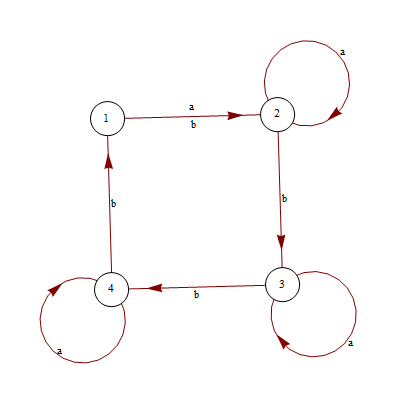
\includegraphics[width=0.75\textwidth]{rysunek1}
    \caption{Synchroniczny automat}
    \label{fig:rysunek1}
\end{figure}

{\L}atwo mo\.{z}emy sprawdzi\'{c}, \.{z}e s{\l}owem resetuj\k{a}cym automat na rysunku \ref{fig:rysunek1} jest \textit{abbbabbba}, co r\'{o}wnowa\.{z}nie mo\.{z}emy zapisa\'{c} \textit{a$b^{3}$a$b^{3}$a}. Pos{\l}ugujac si\k{e} tym s{\l}owem zawsze \'{s}cie\.{z}ka sko\'{n}czy si\k{e} na wierzcho{\l}ku drugim.\\
\\
\textbf{1}$\xrightarrow{a}$2$\xrightarrow{b}$3$\xrightarrow{b}$4$\xrightarrow{b}$1$\xrightarrow{a}$2$\xrightarrow{b}$3$\xrightarrow{b}$4$\xrightarrow{b}$1$\xrightarrow{a}$\textbf{2}\\
\textbf{2}$\xrightarrow{a}$2$\xrightarrow{b}$3$\xrightarrow{b}$4$\xrightarrow{b}$1$\xrightarrow{a}$2$\xrightarrow{b}$3$\xrightarrow{b}$4$\xrightarrow{b}$1$\xrightarrow{a}$\textbf{2}\\
\textbf{3}$\xrightarrow{a}$3$\xrightarrow{b}$4$\xrightarrow{b}$1$\xrightarrow{b}$2$\xrightarrow{a}$2$\xrightarrow{b}$3$\xrightarrow{b}$4$\xrightarrow{b}$1$\xrightarrow{a}$\textbf{2}\\
\textbf{4}$\xrightarrow{a}$4$\xrightarrow{b}$1$\xrightarrow{b}$2$\xrightarrow{b}$3$\xrightarrow{a}$3$\xrightarrow{b}$4$\xrightarrow{b}$1$\xrightarrow{b}$2$\xrightarrow{a}$\textbf{2}\\
\\

%% można ewentualnie dopisać o tym co znaczą kolejne stany w automacie Ashby (2-3 strona opracowania, Singing and Laughting)

Rozwa\.{z}my teraz troszk\k{e} bardziej rozbudowany przyk{\l}ad, tak zwany automat Ashby. Tutaj mamy tyle samo stan\'{o}w co wcze\'{s}niej  Q = \textbraceleft 00, 01, 10, 11\textbraceright, lecz ilo\'{s}\'{c} liter w alfabecie zosta{\l}a zwi\k{e}kszona do czterech. $\Sigma$ = \textbraceleft a, b, c, d\textbraceright.

%% Rysunek 2
\begin{figure}[h]
    \centering
    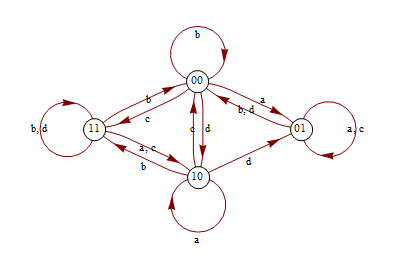
\includegraphics[width=0.75\textwidth]{rysunek2}
    \caption{Automat Ashby}
    \label{fig:rysunek2}
\end{figure}

Rozwa\.{z}aj\k{a}c s{\l}owo \textit{acb} szybko stwierdzimy, \.{z}e jest ono s{\l}owem resetuj\k{a}cym automat przedstawiony na rysunku \ref{fig:rysunek2}\\
\\\\
\textbf{00}$\xrightarrow{a}$01$\xrightarrow{c}$01$\xrightarrow{b}$\textbf{00}\\
\textbf{01}$\xrightarrow{a}$01$\xrightarrow{c}$01$\xrightarrow{b}$\textbf{00}\\
\textbf{10}$\xrightarrow{a}$10$\xrightarrow{c}$00$\xrightarrow{b}$\textbf{00}\\
\textbf{11}$\xrightarrow{a}$01$\xrightarrow{c}$00$\xrightarrow{b}$\textbf{00}\\
\\


\end{document}
